%!TEX root = paper.tex
In this work, we produced a whole-brain resting state functional connectome as follows.
First, $347$ non-overlapping spherical nodes are placed throughout the entire brain in a regularly-spaced grid pattern, with a spacing of $18\times 18 \times 18$ mm; each of these nodes represents a pseudo-spherical ROI with a radius of $7.5$ mm, which encompasses $33$ voxels (the voxel size is $3\times 3\times 3$ mm).
For a schematic representation of the parcellation scheme, see Fig.~\ref{fig:roi,grid,slice}.
Next, for each of these nodes, a single representative time-series is assigned by spatially averaging the BOLD signals falling within the ROI.
Then, a cross-correlation matrix is generated by computing Pearson's correlation coefficient between these representative time-series.
Finally, a vector~\x of length $\binom{347}{2}=60,031$ is obtained by extracting the lower-triangular portion of the cross-correlation matrix.
This vector $\x\in\reals^{60,031}$ represents the whole-brain functional connectome, which serves as the feature vector for disease prediction.

The grid-based scheme for brain parcellation used in this work provides numerous advantages. 
Of note, this approach has been validated in previous studies \citep{Sripada:2013,Sripada:2013b,Sripada:2014}. 
Furthermore, the uniformly spaced grid is a good fit with our implementation of fused Lasso and GraphNet, as it provides a natural notion of nearest-neighbor and ordering among the coordinates of the connectome. 
This property also turns out to be critical for employing our optimization algorithm, which will be discussed in Sec.~\ref{subsec:optim}. 
This is in contrast to alternative approaches, such as methods that rely on anatomical \citep{AAL:2002,Zeng:2012} or functional parcellation schemes \citep{Dosenbach:2010}. 
Anatomical parcellations in particular have been shown to yield inferior performance to alternative schemes in the literature \citep{Power:2011}. 
Additionally, grid-based approaches provide scalable density: there is a natural way to increase the spatial resolution of the grid when computational feasibility allows. 
In particular, to increase node density, one could reduce the inter-node distance and also reduce the node size such that suitable inter-node space remains. 
This scalable density property turns out to be quite important, as our grid-based scheme is considerably more dense than standard functional parcellations (\eg, \cite{Dosenbach:2010, Shirer:2011}) that use as many as several hundred fewer nodes, and thus have tens of thousands fewer connections in the connectome.  
Finally, the use of our grid-based scheme naturally leaves space between the nodes. 
While on the surface this may appear to yield incomplete coverage, this is in fact a desirable property to avoid inappropriate inter-node smoothing. 
This may result as a function of either the point-spread process of fMRI image acquisition or be introduced as a standard preprocessing step. 
In recognition of these advantages, we have elected to use a grid scheme composed of pseudo-spherical nodes spaced at regular intervals.

One pragmatic advantage of using an \apriori parcellation scheme as opposed to one that combines parcellation and connectome calculation is that it permits the usage of a grid, and thus yields all the advantages outlined above. 
Moreover, it allows for easier comparison across studies since an identical (or at least similar) parcellation can be brought to bear on a variety of connectomic investigations. 
Secondly, while an approach that embeds both parcellation and connectome calculation in a single step may be suitable for recovering a more informative normative connectome, it would not necessarily be appropriate for recovering discriminative information about diseases in the connectome unless features were selected based on their disease-versus-healthy discriminative value. 
This approach, however, would require nesting parcellation within cross validation and would lead to highly dissimilar classification problems across cross validation folds and present challenges to any sort of inference or aggregation of performance. 
In light of these challenges, we have elected to use our \apriori grid-based scheme.

%%%%%%%%%%%%%%%%%%%%%%%%%%%%%%%%%%%%%%%%%%%%%%%%%%%%%%%%%%%%%%%%%%%%%%
\renewcommand{\imwidth}  {0.2425\linewidth}
\renewcommand{\imwidthh}  {0.19\linewidth}
\begin{figure}[t!]
	\centering
	\textbf{\large{Grid-based Brain Parcellation Scheme with $\bmath{347}$-nodes}} \vspace{8pt}\\
	\begin{subfigure}[t]{\imwidth}
		\centering
		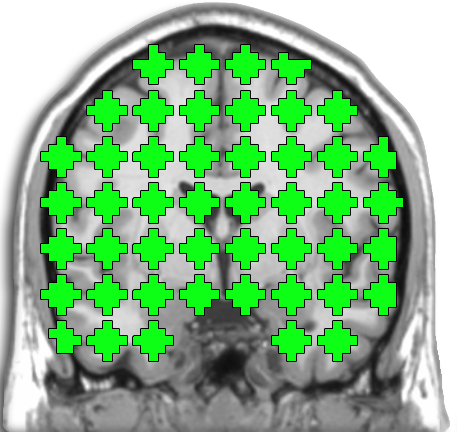
\includegraphics[height=100pt]{roi_slice_cor.png}
		\caption{Coronal}
	\end{subfigure}\hspace{12pt}
	\begin{subfigure}[t]{\imwidth}
		\centering
		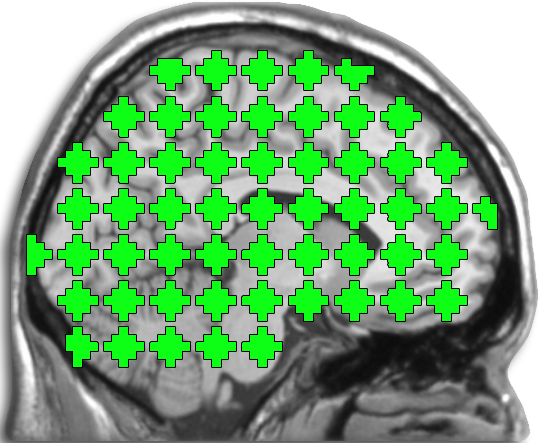
\includegraphics[height=100pt]{roi_slice_sag.png}
		\caption{Sagittal}
	\end{subfigure}\hspace{12pt}
	\begin{subfigure}[t]{\imwidth}
		\centering
		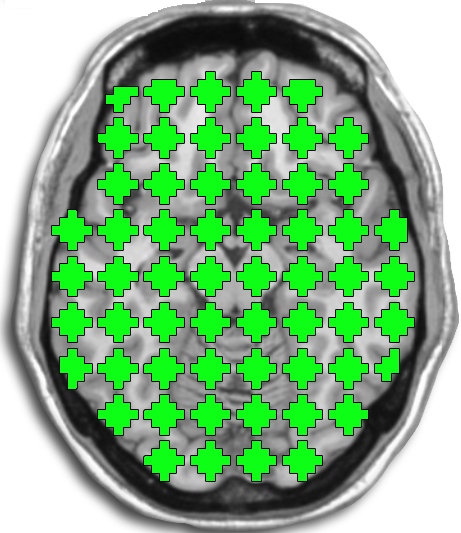
\includegraphics[height=100pt]{roi_slice_axi.png}
		\caption{Axial}
	\end{subfigure}
	\begin{subfigure}[t]{\imwidthh}
		\centering
		\raisebox{15pt}{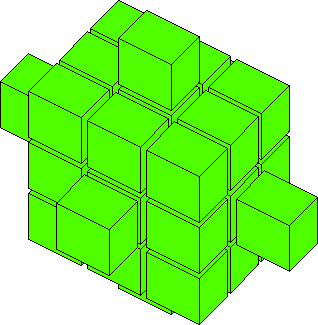
\includegraphics[height=60pt]{roi_pic}}
		\caption{Node (33 voxels)}
	\end{subfigure}
	\caption{
	Coronal, sagittal, and axial slices depicting the coverage of our brain parcellation scheme along with $3$-D rendering of one pseudo-sphereical node. 
	Each contiguous green region represents a pseudo-spherical node representing an ROI containing $33$-voxels.
	Overall, there are $347$ non-overlapping nodes placed throughout the entire brain.
	These nodes are placed on a grid with $18$ mm spacing between node centers in the $X$, $Y$, and $Z$ dimensions.
	}
	\label{fig:roi,grid,slice}
\end{figure}
